\documentclass{sig-alternate-05-2015}
\usepackage{enumerate} 

\begin{document}

\doi{NA}
\isbn{NA}

\title{Automated web application testing: where it has been and where it is going}

\numberofauthors{1} 
\author{
\alignauthor
Timothy Goodrich\\
\affaddr{North Carolina State University}\\
\email{tdgoodri@ncsu.edu}
}

\maketitle
\begin{abstract}
As programs grow larger and larger, testing them becomes more difficult. To some point a human can manually test the software project, but eventually the project becomes too large and complex to test by hand. Therefore \emph{automated testing} has become a very active area of research in recent years. 

Unfortunately, not all software lends itself to automated testing, such as \emph{web applications}. A web application dynamically generates content in response to the interacting user, creating problems for testing such as (a) not having a uniform input/output format across web applications, (b) not having a clearly defined set of possible interactions a user could have at a given web page, and (c) not having a discrete/recognizable number of good outcomes (e.g. rendered pages). These problems make web applications very difficult to test.

This survey centers around problems and solutions introduced in N. Alshahwan and M. Harman's ``Automated web application testing using search based software engineering,'' looking at the past results that these authors utilize and the future work that has extended these results.
\end{abstract}

\keywords{Web applications; Automated test generation; Search-based software engineering}

\section{Introduction}
``Test case generation is among the most labour-intensive tasks in software testing and also one that has a strong impact on the effectiveness and efficiency of software testing'' note Anand et al. \cite{anand2013orchestrated} in the introduction to their survey on automated test generation. In this context, dynamic content applications (e.g. web applications) are the worst of the worst for testing: a vast array of user inputs, content formats, and content outputs presents quite a complex problem. Worse, web applications are open to the whole internet of users, a single bug in thousands of lines of code could lead to a DoS attack or a SQL injection. Therefore developing automated tests for web applications is an important problem. 

This report is centered around a paper by N. Alshahwan and M. Harman, ``Automated web application testing using search based software engineering,'' where the authors present a method for generating tests for PHP-based web applications, the difficulties they faced, and the open problems left for future research. To examine the full context of this work we will examine four papers from the past that Alshahwan et al. cite, and three papers in the future that cite the work of Alshahwan et al. From the start, we note that four common themes will appear:

\begin{enumerate}[\bf \text{Theme} 1.]
\item Automated test generation is computationally difficult and requires heuristics designed specifically for complex problems (e.g. search-based techniques).
\item Test generation heuristics require well-defined decisions (features) and objectives. For functional values (e.g. coverage threshold) this is not a problem, but non-functional values (such as general efficiency) present quite the challenge and are very application-specific. 
\item Web applications contain many poorly-defined inputs, outputs, and objectives. 
\item Web application data is rare, fairly homogenous, and few (if any) real benchmarks exist. 
\end{enumerate}

As we examine the core paper and the related works, note how these themes develop and are addressed by specific results.

\section{The core paper}

\subsection{Summary}

Alshahwan et al. \cite{alshahwan2011automated} introduce a handful of new algorithms (implemented in a tool named SWAT) for automatically testing web pages. They test this tool on six PHP-based web pages, yielding a 54\% increasing in branch coverage and 30\% reduction in practical run time complexity. 

\subsection{Keywords}
\begin{itemize}
\item Search-Based Software Engineering (SBSE): Applying metaheuristic search techniques (gradient-ascending, simulated annealing, etc.) to perform typical software engineering tasks (generating software tests, optimizing parameters, etc.).
\item Automated web application testing: Automatically testing web applications involve both static and dynamic analysis, with an emphasis on the latter. Dynamic testing is computationally difficult given the large number of input options for a web page, making it an active area of current research.
\item Static analysis: Static analysis for software testing is where the code is tested without being run (verification). Typical tests include data flow charts and proofreading code.
\item Dynamic analysis: Dynamic analysis for software testing is where the code is tested by being run (validation). Typical tests include checking how user input is handled, and gauging run times and memory usage.
\end{itemize}

\subsection{Identified Problems with Solutions}
In their approach section, the authors spend a good deal of space describing problems with this sort of testing and their proposed solutions. For example: \\

\noindent \textbf{Issue}: Dynamic Typing\\
\textbf{Description}: Web development languages such as PHP, Python and Ruby are dynamically typed. All variables are initially treated as strings. If used in an arithmetic expression, they are treated as numeric at that operation. However, the same input can be treated as numeric in one expression and as a string in a different expression within the same script. This makes it hard to decide the type of variables involved in a predicate, posing a problem when deciding which fitness function to use.\\
\textbf{Solution}: To solve this problem, types of variables are checked dynamically at run-time using built-in PHP functions and then directed to the appropriate fitness function. \\

In total, the problems identified and fixed are:
\begin{itemize}
\item Interface determination: Interfaces are not uniformly defined between applications and languages. The authors' solution is to perform static analysis to identify the variables that are GET, POST, and REQUESTed, then providing these inputs as parameters to the tool. A similar version of this technique was used in \cite{halfond2009precise}. 
\item Dynamic typing. Variables in web languages are dynamically typed, meaning they keep variable values as strings until an operation requires another data type (e.g. casting into ints for addition). The authors fix this problem by dynamically checking the variable types with built-in PHP functions and using the appropriate fitness functions.
\item User simulation: Typically a user is presented with top-level pages that he or she then navigates, and content is generated client-side and rendered to the user; identifying these top-level pages is non-trivial. The authors' solution is to treat every file not included in another file as a top-level page. 
\item Dynamic includes: PHP supports including files dynamically, where the filename is determined at run time. The authors' solution is to ``approximate'' these include variables by including every file that could possibly be a value for these variables. This technique has been previously used by \cite{wassermann2007sound}.
\end{itemize}

\subsection{Tools and Techniques}
With these problems handled, the authors are able to establish a novel test generation algorithm and variants, implemented with \cite{bouwersphp, bravenboer2008stratego}. The full SWAT tool's architecture is visualized in Figure \ref{fig:swat}: 

\begin{figure}[!h]
\centering
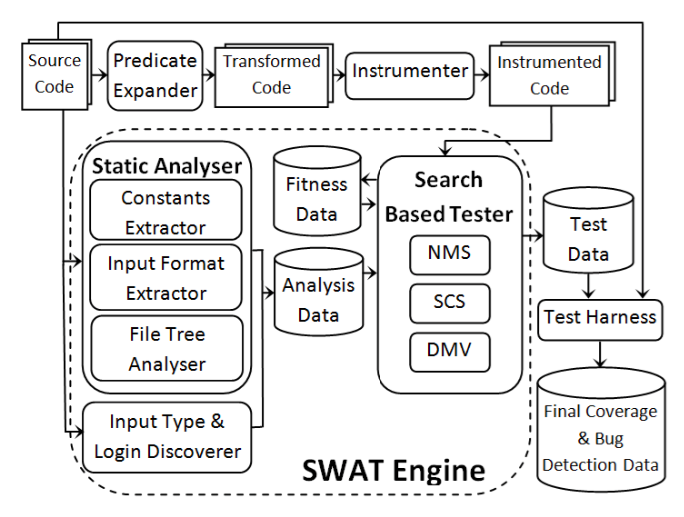
\includegraphics[width=3in]{images/swat.png}
\label{fig:swat}
\caption{The SWAT architecture from \cite{alshahwan2011automated}.}
\end{figure}

Of note are the following details:
\begin{itemize}
\item Broad Test Generation Algorithm: Korel's hill climbing variant is used, which mutates a single decision at a time, and has a mechanism for preventing ``over shooting'' when close to optimal \cite{korel1990automated}.  Furthermore, the code branches that are tracked are either (a) traversed immediately or (b) marked as ``reached'' and traversed later. This choice reduces computation by eliminating the need for ``approach distances''  \cite{mcminn2004search}, but is also not novel \cite{michael2001generating}. See Algorithm 1 in Appendix A for more details. 
\item Mutation Subroutine: If no improvement happened last time, then a new random input is generated. If the last decision that was modified decreased the overall fitness then a new decision is selected, otherwise the decision's ``climbing speed'' is accelerated.  See Algorithm 2 in Appendix A for more details. 
\item Three novel seeding methods for the mutation subroutine are introduced and evaluated: 

\begin{enumerate}
\item Near Miss Seeding (NMS): If a decision was changed and it optimized the fitness of a branch other than the current one then it is considered a ``near miss'' and is recorded for later exploitation. 
\item Static Constant Seeding (SCS): SCS is where constants are used to initialize a new candidate instead of completely random values. This technique was introduced in \cite{alshraideh2006search} in the context of traditional applications and adapted to the web application format by the Alshahwan et al. 
\item Dynamically Mixed Value Seeding (DMV): When this hill climbing algorithm is run, a database is maintained of constants associating certain input with certain output (e.g. selecting the ``Help'' button from the overhead menu will always lead to the help page, regardless of previous input). These associations are then used when mutating to provide optimal coverage: the algorithm knows which web pages have been covered and has a rough idea of what inputs led to this page, so new inputs are chosen to lead to new web pages. This DMV seeding is a particularly novel ``kernel'' to the SWAT tool and addresses both the problem of test generation coverage and the problem of broadly-defined web page inputs/outputs. 
\end{enumerate}
\end{itemize}

\subsection{Data}
This paper uses a dataset introduced earlier in Artzi et al \cite{artzi2010finding}, consisting of six open source PHP web applications:

\begin{figure}[!h]
\centering
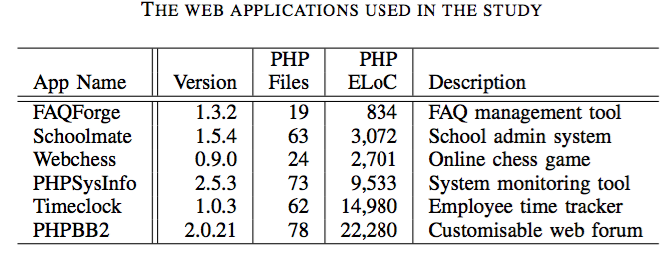
\includegraphics[width=3in]{images/php.png}
\label{fig:php}
\caption{The PHP web application input corpus from \cite{alshahwan2011automated}.}
\end{figure}

Unfortunately, Artzi et al. provide little motivation for introducing this dataset other than noting that they are freely available on SourceForge \cite{sourceforge}. Furthermore, the only real distinction in this dataset seems to be the split between small programs (FAQForge and Webchess with 19-24 PHP files) and medium-sized programs (Schoolmate, PHPSysInfo, Timeclock, and PHPBB2 with 62-78 files). So in some sense there is little motivation for using this dataset, other than because previous PHP-test generation algorithms have used this dataset. 


\subsection{Results}
Visualized in Figure \ref{fig:results}, the results fairly conclusively show that DMV seeding is by far the victor in terms of covered branches and in actual bugs (faults) found. A  comparison to the previous work \cite{artzi2010finding} is not given, potentially due to the latter not containing timing data (we expect an explicit-state model checker algorithm to perform better than a symbolic model checker because all states are explicitly checked, therefore solution quality alone is not a fair comparison). 

\begin{figure*}
\centering
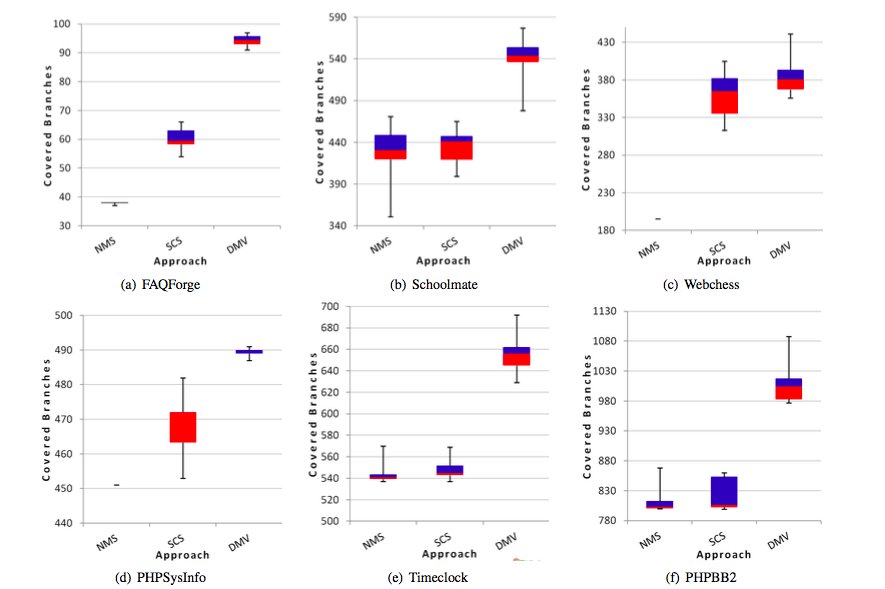
\includegraphics[width=6in]{images/results1.png}
\vspace{0.5in}

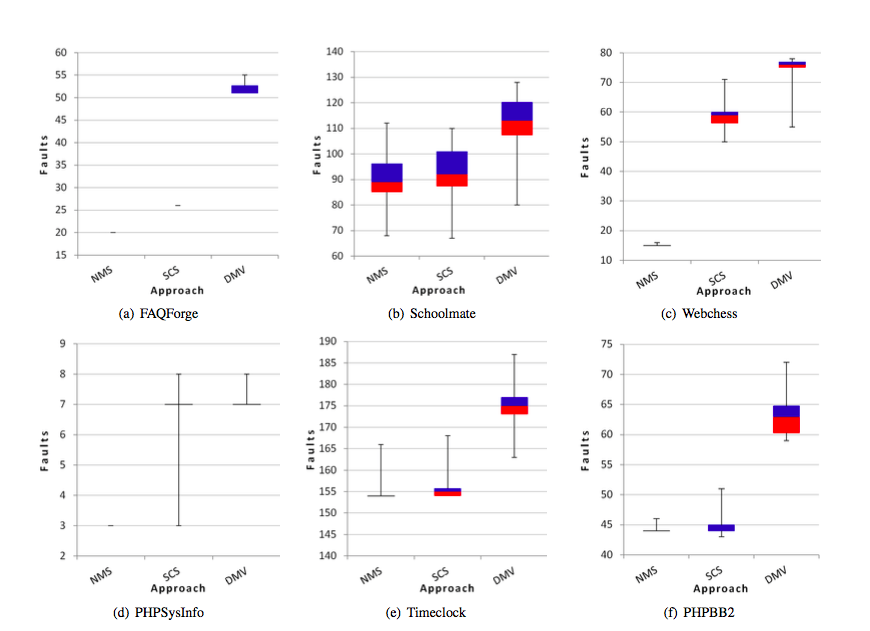
\includegraphics[width=6in]{images/results2.png}
\label{fig:results}
\caption{Results (in terms of coverage and in faults found) of 30 runs of each of the 3 seeding methods for the 6 datasets from \cite{alshahwan2011automated}.}
\end{figure*}

\subsection{Open Problems}
While this work showed that dynamically tracking which inputs led to which outputs (the DMV seeding) was highly useful, some open problems still exist:

\begin{itemize}
\item Lack of tool automation. While the optimization process itself was automated, the tool itself was not and manually needed to be set up with the web application (a non-trivial process). Further work in unifying the input/output of web applications is needed for this automation to become a reality. 
\item Generalizing beyond PHP. While this tool worked well on the six PHP web application, PHP is a very specific language and these six web pages is a fairly small testing corpus. Generalizing both of these factors is an open problem.
\item More intricate solutions to the preprocessing problems. The authors made several naive choices in handling the initial problems presented in preprocessing, such as importing all possible included files. Making more intricate choices here is desirable, both for run time purposes and automation purposes. 
\end{itemize}





\section{Related Works: The Past}


\subsection{Dynamic test input generation for web applications (2008)}

\subsubsection{Summary}
Wassermann et al \cite{wassermann2008dynamic, wassermann2007sound} address differences between typical application (C or Java) testing and web application (PHP or Javascript) testing. Specifically, they propose using concolic (concrete + symbolic) testing for web applications, and test their methods on three PHP web sites (Mantis, Mambo, and Utopia News) in the context of detecting SQL injections. Little result statistics are given, but their approach generally seems to work.  

\subsubsection{Keywords}

\begin{itemize}
\item Automated web application testing: Automatically testing web applications involve both static and dynamic analysis, with an emphasis on the latter. Dynamic testing is computationally difficult given the large number of input options for a web page, making it an active area of current research.
\item Dynamic test generation: Dynamic testing gauges how well a piece of software responds to input, and generating sufficient tests is difficult (especially for web pages). Generating such tests is an active area of research.
\item Test coverage: The coverage of a test measures how many branches (paths) a test covers in a piece of software. Different measures exist, such as lines covered, function calls covered, etc.
\item Concolic testing framework: Concolic (concrete + symbolic) testing is a hybrid technique for performing both symbolic execution (``theoretical'') and concrete execution (``practical'') with real inputs.
\end{itemize}

\subsubsection{Relevance to the Core Paper}
Alshahwan et al. \cite{alshahwan2011automated} cited this paper in the context of applying symbolic execution to source code (specifically web applications), but noted that the results were limited to function calls with SQL queries due to their interest in detecting SQL injection vulnerabilities. 

\subsubsection{Broader Relevance}
Ultimately, this paper did not contribute much to the web application testing community, seemingly because their results were very niche (SQL injection vulnerability detection) compared to the full testing that most researchers seem interested in. The three datasets used in this paper did not appear again in any subsequent papers I read or cited. 

`
\subsection{A systematic review of search-based testing for non-functional system properties (2009)}

\subsubsection{Summary}
Afzal et al \cite{afzal2009systematic} provide a systematic survey paper of search-based testing techniques for non-functional properties. They identified Safety, Usability, Security, Quality of Service, and Execution Time as the non-functional properties examined in the literature, with the usual search-based techniques appearing (genetic algorithms, simulated annealing, hill climbing, etc.). The authors did not provide a recommendation on which technique to use for a given non-functional property, but rather provided the names of researchers who had applied $x$ technique to $y$ functional property, and noted this evolution over time. 

\subsubsection{Keywords}

\begin{itemize}
\item Search-Based Software Engineering (SBSE): Applying metaheuristic search techniques (gradient-ascending, simulated annealing, etc.) to perform typical software engineering tasks (generating software tests, optimizing parameters, etc.).
\item Test adequacy criterion: Test adequacy criteria is a set of requirements that evaluate whether a set of tests are sufficient or not. These criteria could include requirements about percent code coverage, which inputs are tested, etc.
\item Non-functional properties/requirements: Non-functional properties/requirements indicate whether a piece of software is behaving correctly, but cannot specify particular behaviors. For example, properties such as speed, size, throughput, power consumption and bandwidth are non-functional, and the software requirements might specify ranges for each property; but the requirement cannot specify exact values.
\item Fitness function: A fitness (objective) function summarizes a single attribute of a solution, particularly one used to gauge how ``good'' a solution is. For example, run time is a typical fitness function for algorithms.
\end{itemize}

\subsubsection{Relevance to the Core Paper}
Alshahwan et al. \cite{alshahwan2011automated} cited this paper as an example of search-based techniques applying to both functional (natural) and non-functional (non-trivial) properties. However, none of the particular non-functional properties were used in web site testing, so the results were not directly applicable. 

\subsubsection{Broader Relevance}
As a survey paper, this work is fantastic in overviewing which techniques were used by which groups of authors on specific properties. At the time this report was written, the paper had over 200 citations.

\subsection{Precise interface identification to improve testing and analysis of web applications (2009)}

\subsubsection{Summary}
Halfond et al \cite{halfond2009precise} recognized that web applications have varied and ill-defined interfaces, making it a problem to create testing tools. They propose a form of symbolic execution used to abstract away these implementation details and provide a nice interface for a test generator. They test this symbolic executer on several applications, including test-input generation, penetration testing, and invocation verification.  

\subsubsection{Keywords}

\begin{itemize}
\item Program testing: Performing an investigation to gauge the quality of a piece of software, especially when used under specific conditions.
\item Automated web application testing: Automatically testing web applications involve both static and dynamic analysis, with an emphasis on the latter. Dynamic testing is computationally difficult given the large number of input options for a web page, making it an active area of current research.
\item Symbolic execution: Symbolic execution is a method of checking which (set of) inputs trigger parts of a program to execute, and can be represented graphically as a path. Execution time is typically exponential.
\item Penetration testing: Penetration testing tests if a piece of software (usually a web application) can be exploited, particularly with malicious user input.
\end{itemize}

\subsubsection{Relevance to the Core Paper}
Alshahwan et al \cite{alshahwan2011automated} used a similar approach in handling interface determination by performing static analysis over the GET, POST, and REQUEST statements. The authors also note that Halfond et al's specific approach was limited to Java applications, whereas Alshahwan et al. applied the same idea to PHP applications. Despite the specifics, however, it seems that Halfond et al's approach was necessary for Alshahwan et al's results. 

\subsubsection{Broader Relevance}
More broadly, Halfond et al do a good job of establishing a rigorous way of handling ill-defined input with an abstract layer, and all future work on this question builds off of their work. Of all the papers in this survey, this paper seemed the most universally respected and useful. 


\subsection{Finding Bugs in Web Applications Using Dynamic Test Generation and Explicit-State Model Checking (2010)}

\subsubsection{Summary}
Artzi et al \cite{artzi2010finding} solve basically the same problem as Alshahwan et al \cite{alshahwan2011automated}, but with explicit-state model checking instead of symbolic model checking. The same six PHP web applications are used, and the results are an upper bound for the much faster symbolic model checker, as expected. In some sense, this paper answers the ``Can we test PHP web applications?'', whereas Alshahwan et al's paper answers ``How can we quickly test PHP web applications?''

\subsubsection{Keywords}
\begin{itemize}
\item Program testing: Performing an investigation to gauge the quality of a piece of software, especially when used under specific conditions.
\item Program verification: Program verification checks that the program was written correctly, and is typically associated with static testing.
\item Dynamic test generation: Dynamic testing gauges how well a piece of software responds to input, and generating sufficient tests is difficult (especially for web pages). Generating such tests is an active area of research.
\item Explicit state model checking: Model checking involves testing whether a piece of software meets its specification. Explicit state model checking walks through every possible state explicitly, and typically has exponential run time.
\end{itemize}

\subsubsection{Relevance to the Core Paper}
As mentioned before, this paper seems to be the groundwork for the Alshahwan et al paper. The latter authors note that their work differs in that they are optimizing for \emph{branch coverage}, whereas the former optimized for \emph{statement coverage}. However, the motivation remained the same, and this work was an important first stab at the problem. 

\subsubsection{Broader Relevance}
In a broader context, this paper is eclipsed by the Alshahwan et al paper. Explicit state model checking is the expensive, ``dumb'' way of testing in the classical computational complexity sense (``how do we solve the problem? Try every possible combination!''). Contrastingly, Alshahwan et al's result provides an \emph{intuition} for what seems to be working (the DMV seeds track what is important and so reduce run time without reducing too much solution quality). Artzi et al's result is a stepping stone, then, and not a standalone result that has proven reusable (like Halfond et al's result). 


\section{Related Works: The Future}

\subsection{Software Engineering Meets Evolutionary Computation (2011)}

\subsubsection{Summary}
This paper \cite{harman2011software} is Harman's high-level survey of search-based techniques (specifically with evolutionary components) applied to software engineering problems. Harman emphasizes the exponential increase in the number of annual SBSE publications, and highlights the different software engineering problems that reduce to an optimization problem to be solved with evolutionary computing. 

\subsubsection{Keywords}

\begin{itemize}
\item Evolutionary computation: Evolutionary computation is a class of algorithms that adopt Darwinian principles (e.g. evolution) to generate waves of candidate solutions. Examples include genetic programming, ant-colony optimization, etc.
\item Realistic algorithm: An informal definition, a realistic algorithm can be expected to run in a reasonable amount of time on a reasonable amount of input; exact orders of magnitude will be domain-specific. For example, in theoretical computer science a polynomial-time algorithm is fast, whereas in engineering applications an algorithm needs linear (or log-linear) run time to be useful.
\item Search-Based Software Engineering (SBSE): Applying metaheuristic search techniques (gradient-ascending, simulated annealing, etc.) to perform typical software engineering tasks (generating software tests, optimizing parameters, etc.).
\item Software design: Software design is the process of formalizing a set of specifications, requirements, and constraints that a proposed piece of software will satisfy. These details can be quantitative or qualitative, and typically evolve as the software matures.
\end{itemize}

\subsubsection{Relevance to the Core Paper}
In some sense this paper is the least interesting because it is so high-level. But taking this step back emphasizes one fact: web application testing can and is done with evolutionary computing. The Alshahwan et al paper has ``made it,'' so to say.

\subsubsection{Broader Relevance}
This survey paper does a good job at offering an updated picture of the field portrayed by Afzal et al. Several repeated citations also suggests that there's a strong correlation between ``interesting software engineering problem'' and ``non-functional properties,'' an interesting side-note.  


\subsection{The GISMOE challenge: constructing the pareto program surface using genetic programming to find better programs (2012)}

\subsubsection{Summary}
The GISMOE challenge is a framework proposed by Harman et al \cite{harman2012gismoe} for offering the software developer a choice of coding trade-offs before any code is written. More formally, the software engineering project's decisions and objectives are encoded into an optimization problem, and a Pareto frontier (surface) is generated. By picking any candidate on this surface, the software developer can choose between several tangible trade-offs. This framework's benefits are two-fold: (a) the optimization algorithm does not need to solve the trade-offs itself, so generating a large frontier is almost preferred, and (b) the software developer is not simply presented with a single result, but is offered an entire surface of options. Ultimately, Harman et al hope to fundamentally change how SBSE interacts with humans, resulting in more efficient algorithms and more useful results. 

\begin{figure*}[!h]
\centering
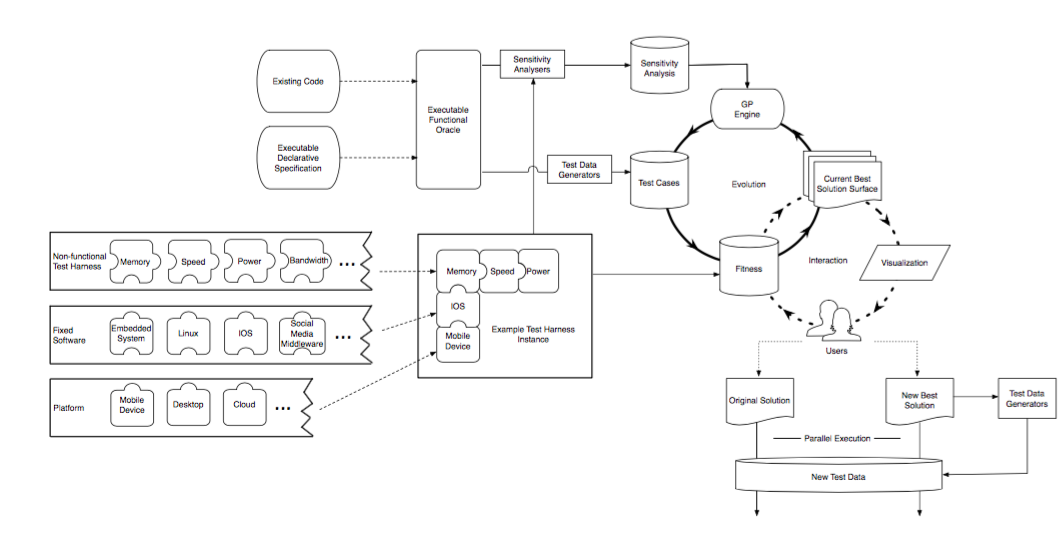
\includegraphics[width=7in]{images/gismoe.png}
\label{fig:gismoe}
\caption{The proposed GISMOE framework from \cite{harman2012gismoe}.}
\end{figure*}

\subsubsection{Keywords}

\begin{itemize}
\item Non-functional properties/requirements: Non-functional properties/requirements indicate whether a piece of software is behaving correctly, but cannot specify particular behaviors. For example, properties such as speed, size, throughput, power consumption and bandwidth are non-functional, and the software requirements might specify ranges for each property; but the requirement cannot specify exact values.
\item Functional properties/requirements: Functional properties/requirements specify exactly what output the software should have.
\item Search-Based Software Engineering (SBSE): Applying metaheuristic search techniques (gradient-ascending, simulated annealing, etc.) to perform typical software engineering tasks (generating software tests, optimizing parameters, etc.).
\item Pareto surface/frontier: In multi-objective optimization, the Pareto surface/frontier is the set of all candidate solutions which are not dominated.
\end{itemize}

\subsubsection{Relevance to the Core Paper}
The GISMOE paper does not mention web application testing explicitly, but rather groups the Alshahwan et al paper in with ``recent SBSE advances'' in general. Again, we see that Harman in particular sees the Alshahwan et al result as strong enough proof that SBSE provides an advantage when generating tests for web applications. 

\subsubsection{Broader Relevance}
GISMOE diverges from the typical description of SBSE in the sense that it does not propose to be an algorithm that takes in a software engineering problem and outputs a solution. Instead, GISMOE could/will be a tool for understanding a problem's fundamental trade-offs and choosing (manually) which objectives it makes sense to optimize/prioritize. This claim can be taken one of two ways. First, GISMOE is too high-level to be useful, i.e. a pseudo-science with no real fundamental results. On the other hand, it could take the existing SBSE field, with all the results cited in this survey, and change around the picture to involve human interaction in a new manner. The GISMOE project might be an interesting work to keep track of over the next several years.

\subsection{An orchestrated survey of methodologies for automated software test case generation (2013)}

\subsubsection{Summary}
Anand et al \cite{anand2013orchestrated} present a survey paper on automated software testing, using the following techniques: (a) structural testing using symbolic execution, (b) model-based testing, (c) combinatorial testing, (d) random testing and its variant of adaptive random testing, and (e) search-based testing. The search-based testing section is written by Mark Harman, Phil McMinn, John Clark and Edmund Burke, and cites dozens of applications (including web application testing). 

\subsubsection{Keywords}

\begin{itemize}
\item Dynamic test generation: Dynamic testing gauges how well a piece of software responds to input, and generating sufficient tests is difficult (especially for web pages). Generating such tests is an active area of research.
\item Search-Based Software Engineering (SBSE): Applying metaheuristic search techniques (gradient-ascending, simulated annealing, etc.) to perform typical software engineering tasks (generating software tests, optimizing parameters, etc.).
\item Non-functional properties/requirements: Non-functional properties/requirements indicate whether a piece of software is behaving correctly, but cannot specify particular behaviors. For example, properties such as speed, size, throughput, power consumption and bandwidth are non-functional, and the software requirements might specify ranges for each property; but the requirement cannot specify exact values.
\item Functional properties/requirements: Functional properties/requirements specify exactly what output the software should have.

\end{itemize}

\subsubsection{Relevance to the Core Paper}
As seems to be the theme with the future papers, no new results are made in automated web testing; instead, the current results are cited and ``web application testing'' is cited as an area where SBSE has suceeded. 

\subsubsection{Broader Relevance}
Whereas the Afzal et al survey covered search-based techniques alone, this survey includes search-based techniques as only one of five different options. This survey also emphasizes results and provides recommendations based on effectiveness, whereas the Afzal et al paper concentrated on the trends in metaheuristic usage over time and the clusters of researchers working with these metaheuristics. We see a shift, then: before, the emphasis was on the techniques used and how well they tested different properties. Now we see the emphasis on the question ``What can you \emph{do} with these metaheuristics?'', pushing the limit on what the field as a whole can do. Of note: web application testing appears as an application with a solid solution. 

\section{Commentary}
In this report, we have done the following:
\begin{itemize}
\item Zoomed in on a particular result of search-based techniques applied to generated automated tests for web applications.
\item Noted that while some previous results came close to solving the same problem, no future results have (so far) looked at the same problems. 
\item Also noted that more recent works have happily called ``web application testing'' a tried-and-true area of results.
\end{itemize}

In some sense it seems like this area is stagnant. The existing result is fairly substantial, and the more recent works have no emphasizes any open problems in the area. However, if we want to find some open problems, we need not look too far. Instead, we merely need to add more theory or more applications:
\begin{enumerate}[\textbf{Theory} 1.]
\item The DMV seeding found correlations between conditional branches and input values. Is there a smarter way to keep track of these values? For example, differential evolution \cite{storn1996differential} ``accidentally'' keeps track of best values by not throwing their candidates out. At a high level we can imagine that differential evolution makes a natural fit: we can crossover the common features to candidates so that more branches are explored. Perhaps there are some results to come from looking at DEs. 
\item Tabu search \cite{glover1997tabu} is a general technique for keeping track of previously seen values and ignoring them in a future search, and yet this technique was not mentioned in the Alshahwan et al paper. Why not? This seems like a natural mechanism for seeding the mutations. 
\end{enumerate}

\begin{enumerate}[\textbf{Application} 1.]
\item The PHP datasets used in the papers here were small and not very regular. A six PHP web application dataset was used in two papers, and a three PHP web application dataset was used in another paper with an emphasis on SQL injections. Why stick with PHP if the datasets are so rare and small? One alternative might be to look at Android application repositories \cite{krutz2015dataset, hamasaki2013who}. Android applications offer the same problems as web applications (dynamically generated content, a wide array of user inputs), and dozens of good open source Android datasets exist. Perhaps by extending the current results to these new datasets, new features (good and bad) will be revealed. 
\end{enumerate}

\section{Conclusion}

In conclusion, we have seen how a result begins from a collection of techniques applied to a vague problem (web applications), become concrete (search-based techniques applied to PHP applications), and then become vague in the techniques and specific in the problem (evolutionary computing as a whole applied to specific web applications). In some sense we have seen the lifespan of this result: it was born as a wide array of techniques were applied to a specific problem, and now is written off as an area where SBSE has found results. Curiously, this might be why we have not seen new results in the area of web application testing -- the problem is written off as solved and uninteresting now. Perhaps new datasets will liven up the work, perhaps not. Perhaps new algorithms will lead to more intriguing problems, perhaps not. Either way, we see how research iterates between techniques and problems as the driving force, and how many attempts must be made before a good solution is found.

\newpage
\bibliographystyle{acm}
\bibliography{citations} 

\newpage
\appendix
\section{Pseudocode}

\begin{figure}[!h]
\centering
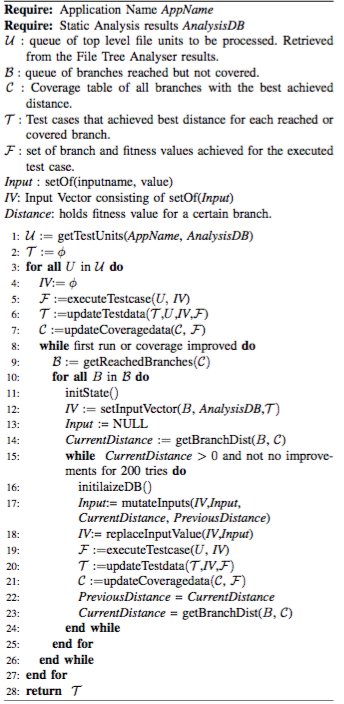
\includegraphics[width=3in]{images/algorithm1.png}
\label{fig:algorithm1}
\caption{Algorithm 1 from \cite{alshahwan2011automated}.}
\end{figure}

\begin{figure}[!h]
\centering
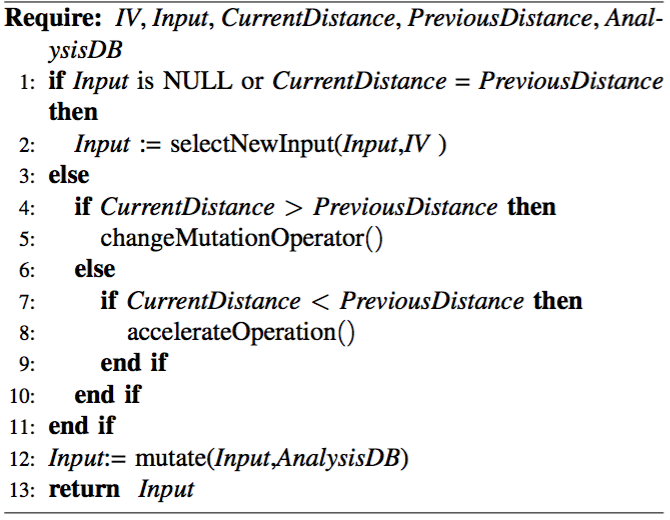
\includegraphics[width=3in]{images/algorithm2.png}
\label{fig:algorithm2}
\caption{Algorithm 2 from \cite{alshahwan2011automated}.}
\end{figure}

\end{document}
